\subsubsection{GPIO. ШИМ}

Для генерации ШИМ можно использовать расположенные на плате Raspberry Pi GPIO контакты.

Для программной генерации ШИМ можно использовать все контакты GPIO, но при таком подходе часть аппаратных ресурсов платформы будет тратиться на генерацию и кодирование импульсов, что влечёт за собой уменьшение производительности всей системы. Для аппаратной генерации ШИМ предназначены контакты GPIO12, GPIO13, GPIO18, GPIO19 Raspberry Pi. В этом случае достигается большая производительность системы и упрощение для разработчика при работе с напряжением на контактах GPIO. Полная карта контактов Raspberry Pi представлена на рисунке~\ref{img:raspberrypi__GPIO_pinout_diagram}.

\begin{figure}[H]
  \centering
  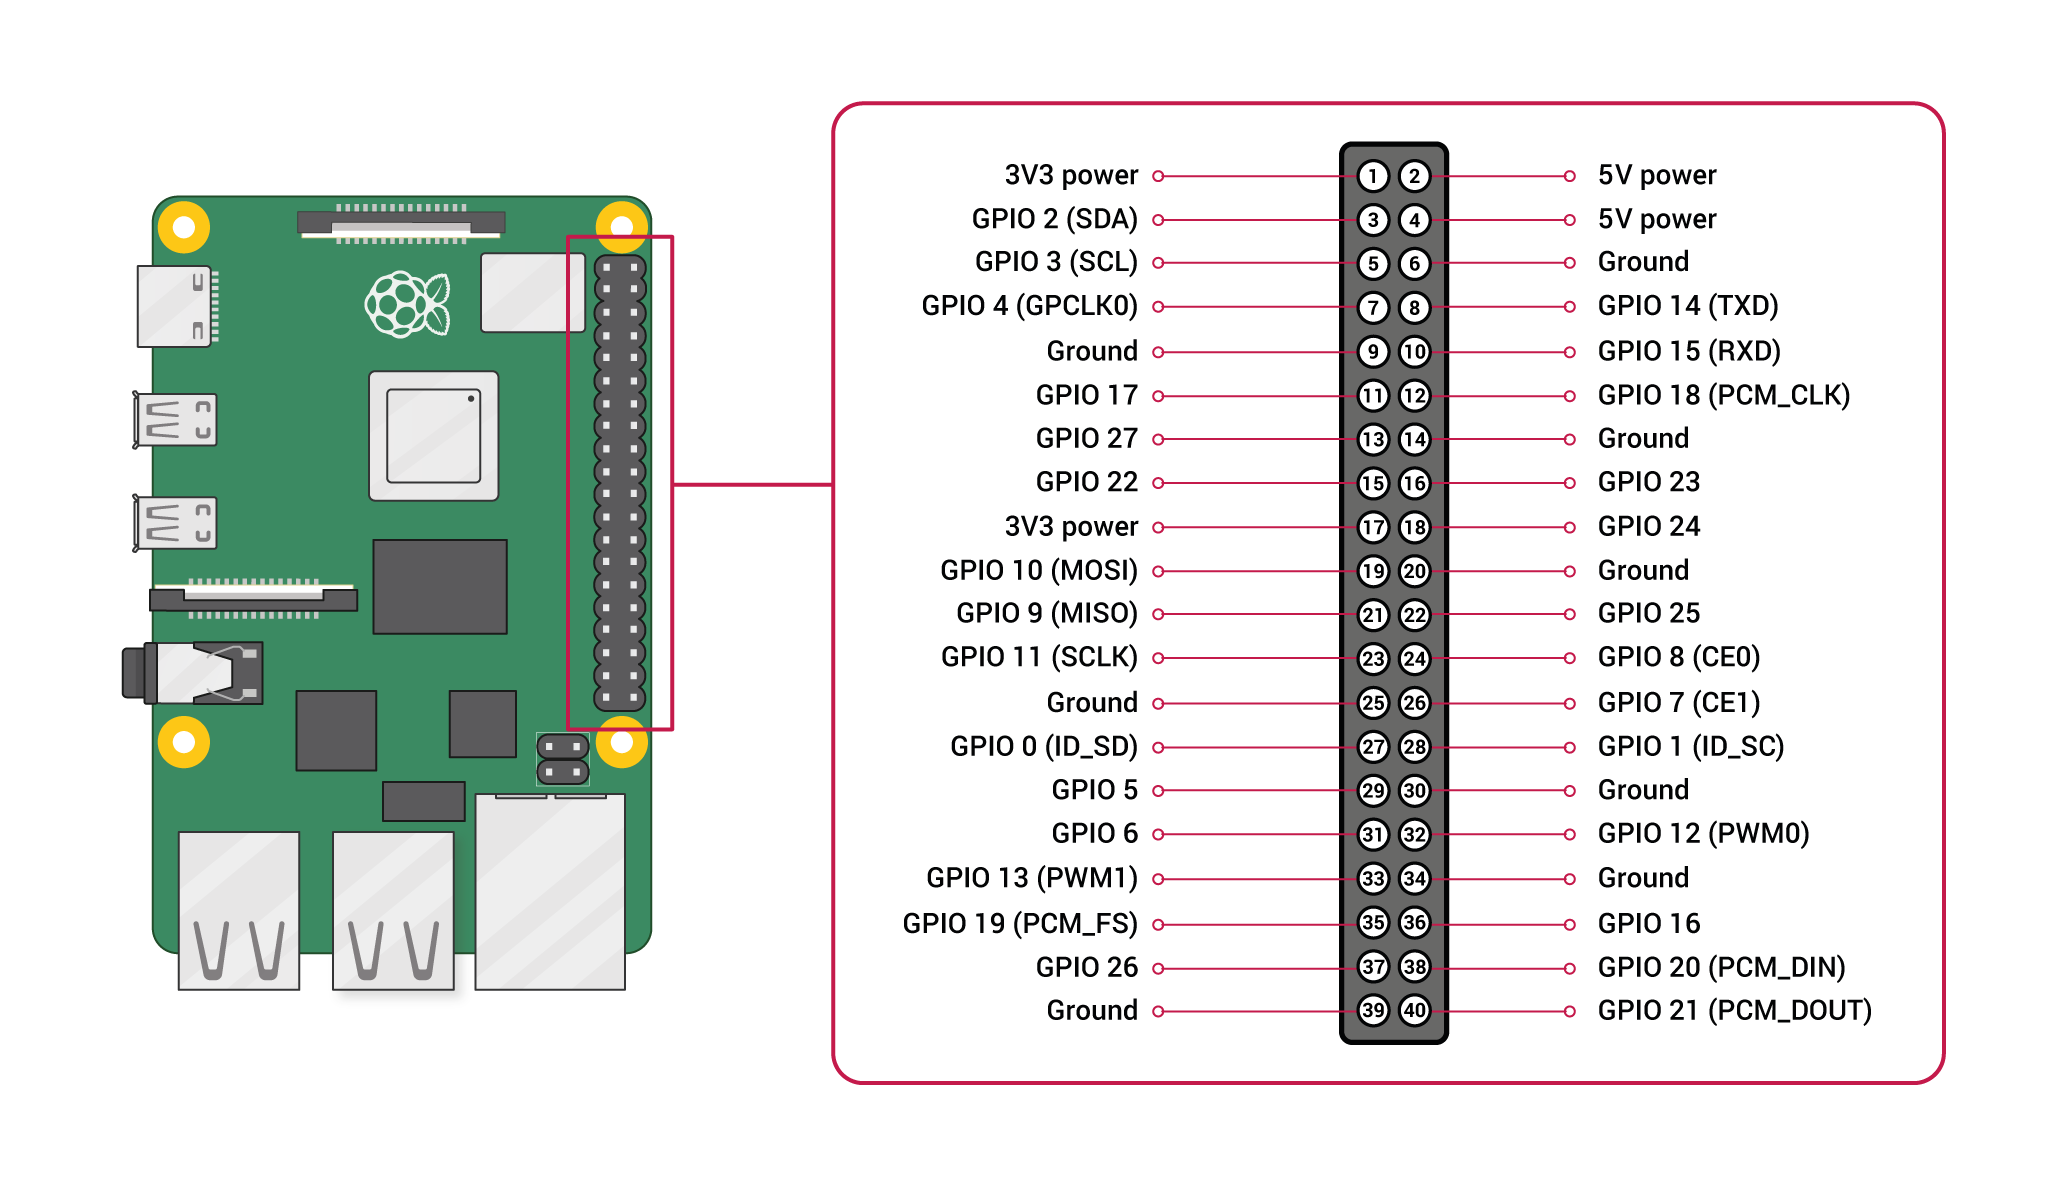
\includegraphics[width=0.9\textwidth]{assets/images/practical/GPIO-Pinout-Diagram.png}
  \caption{Карта GPIO контактов Raspberry Pi}
  \label{img:raspberrypi__GPIO_pinout_diagram}
\end{figure}

Ввиду описанных выше факторов, для генерации ШИМ был выбран контакт GPIO18, обозначен номером 12 на карте~\ref{img:raspberrypi__GPIO_pinout_diagram}. Также, согласно карте GPIO контактов, в качестве контакта заземления был выбран контакт 6.

В следствие этого, был разработан итоговый макет программно-аппаратного комплекса. Макет представлен на рисунке~\ref{img:all__schema}. На макете цифрами отмечены элементы:

\begin{itemize}
  \item 1 -- макетная плата;
  \item 2 -- диод 1N4001, предназначенный для предупреждения повреждений комплекса из-за неправильного подключения питания;
  \item 3 -- элемент питания;
  \item 4 -- одноплатный компьютер Raspberry Pi 3 model B;
  \item 5 -- светодиодная лента WS2812b.
\end{itemize}

\begin{figure}[H]
  \centering
  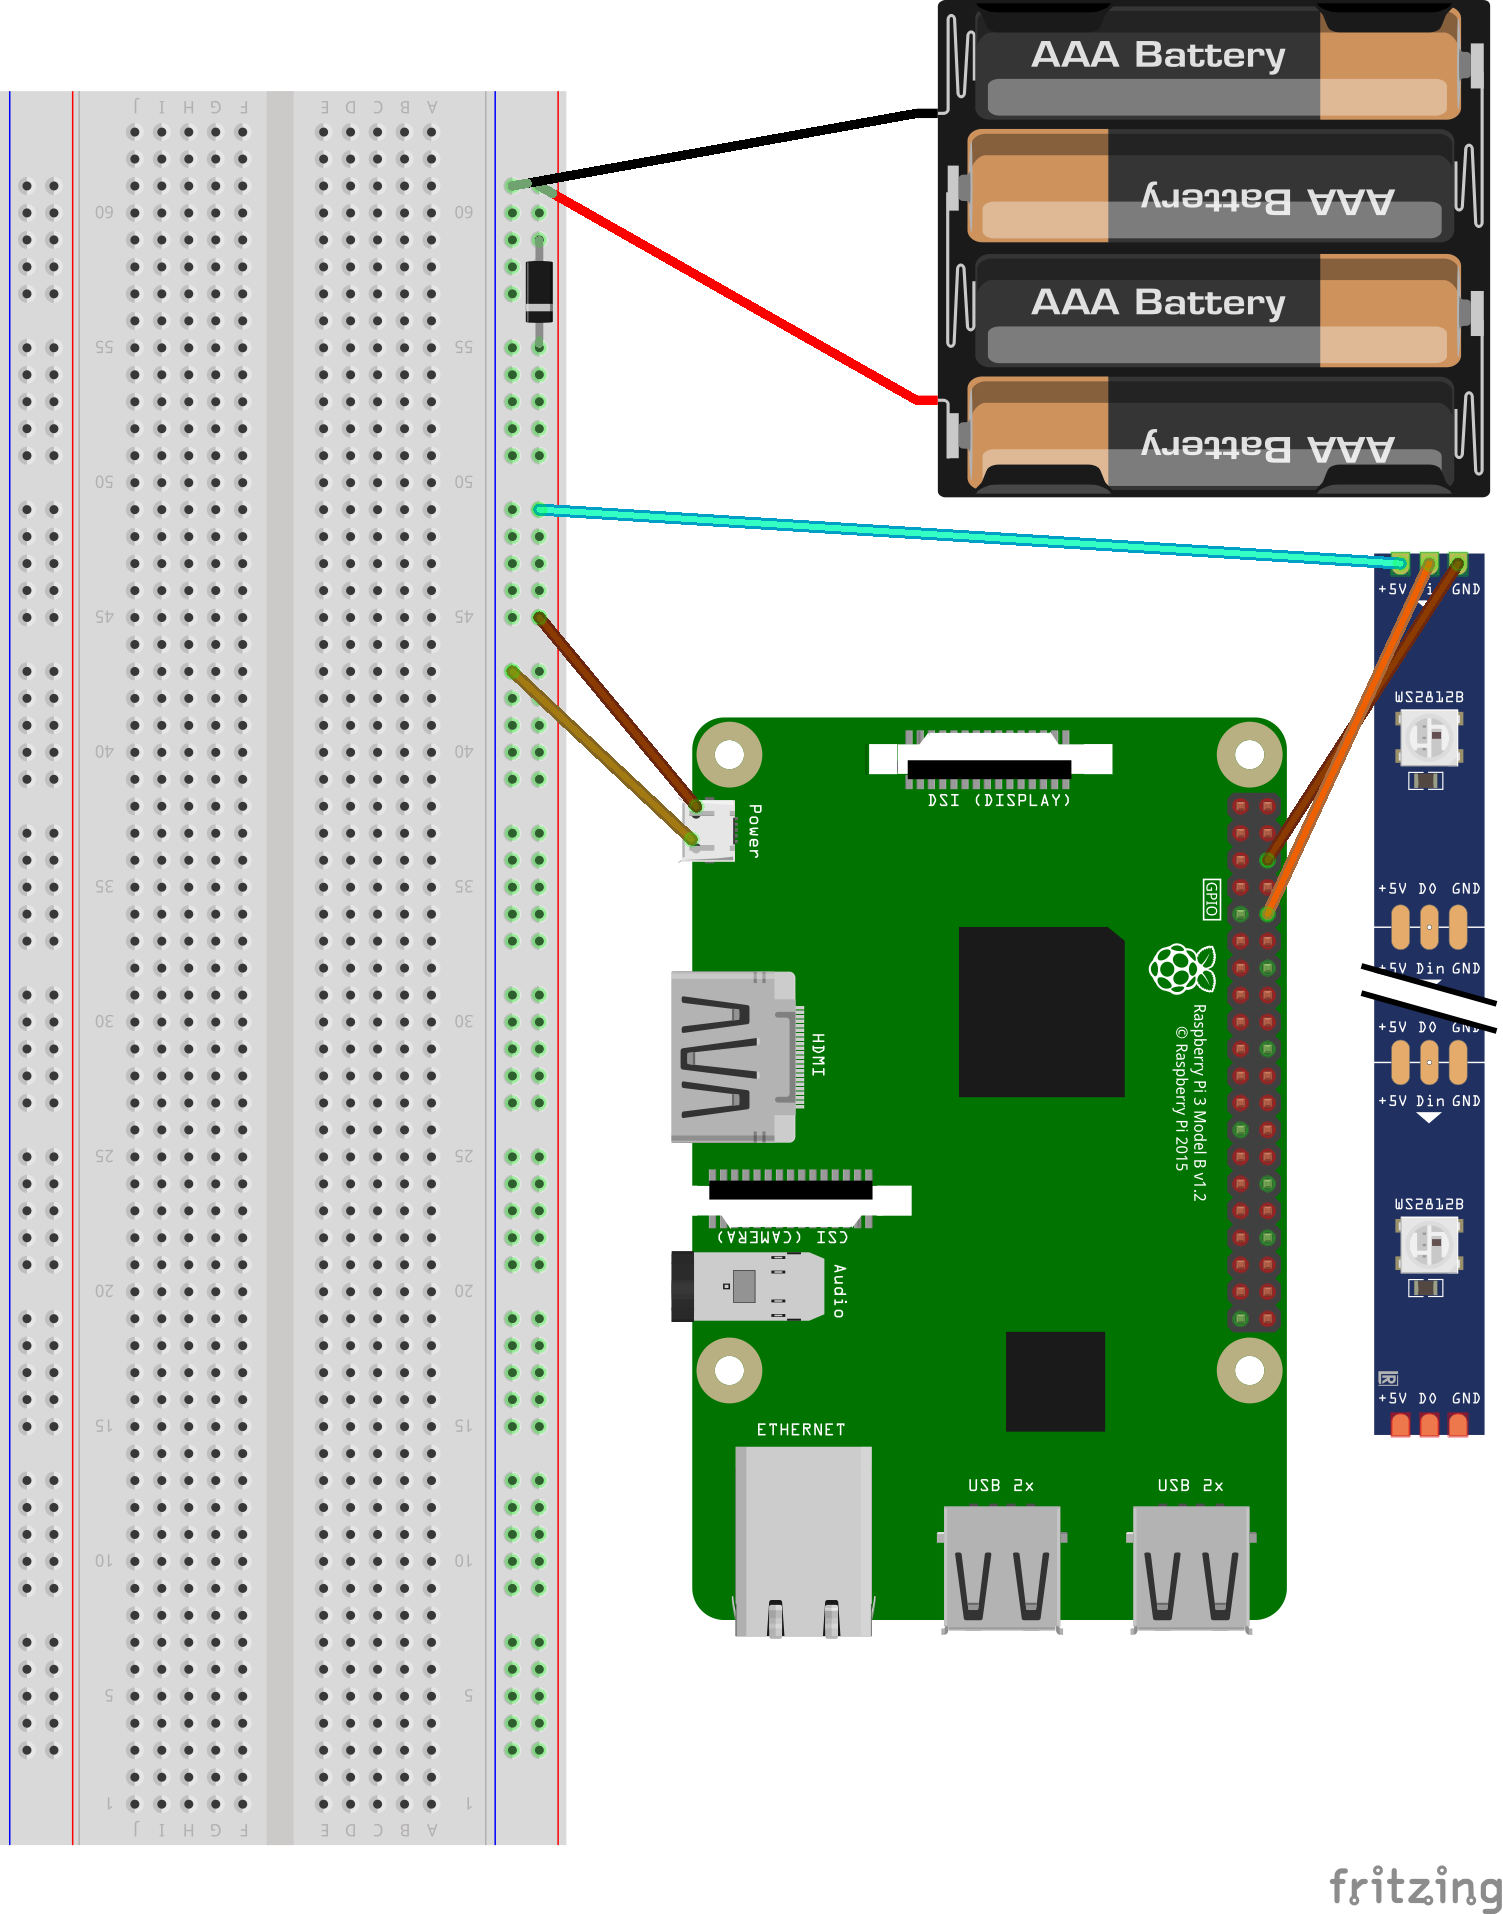
\includegraphics[angle=-90, width=0.9\textwidth]{assets/images/practical/Итоговая архитектура программно-аппаратного комплекса.png}
  \caption{Итоговый макет программно-аппаратного комплекса}
  \label{img:all__schema}
\end{figure}

Согласно макету~\ref{img:all__schema} была собрана и протестирована работоспособность системы. На этом разработку аппаратной части комплекса можно считать завершённой. Собранный комплекс представлен на рисунке~\ref{img:all__hard}.

\begin{figure}[H]
  \centering
  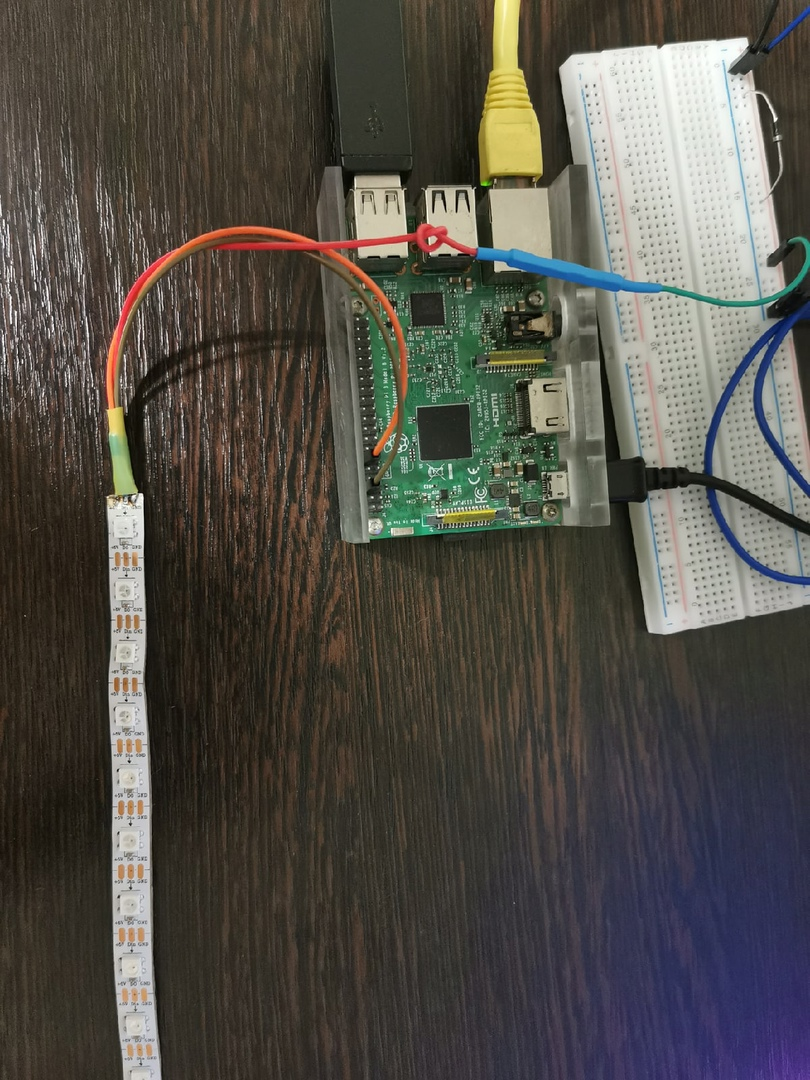
\includegraphics[angle=90, width=0.9\textwidth]{assets/images/practical/Полная схема.jpg}
  \caption{Собранный комплекс}
  \label{img:all__hard}
\end{figure}
